\section{Introduction}
\label{sec:intro}

The emerging paradigm of AI for Science (AI4S) and interdisciplinary studies promises to transform Large Language Models (LLMs) from passive knowledge retrievers into active research assistants capable of cross-domain integration \cite{zhang-etal-2024-comprehensive-survey,zheng-etal-2025-automation}. 
In practice, realistic scientific discovery is rarely a stationary inference; it is an inherently interactive, multi-constraint, and interdisciplinary process.
For instance, material design typically requires synthesizing constraints from compositional analytical \textit{chemistry}, solid-state \textit{physics}, and \textit{financial} cost assessment; similarly, medicinal analysis often interleaves molecular \textit{biology} with \textit{mathematical} estimation and experimental \textit{engineering} \cite{zhang-etal-2024-comprehensive-survey,zheng-etal-2025-automation}.
Such scenarios fundamentally demand that models possess capabilities \textbf{Compositional Generalization in Scientific Knowledge} —\emph{the ability to systematically recombine knowledge from disparate domains to solve complex, interactive problems} \cite{lake2018generalization,keysers2020measuring,gong2026subspacepath}.

\begin{figure}[!t]
    \centering  
    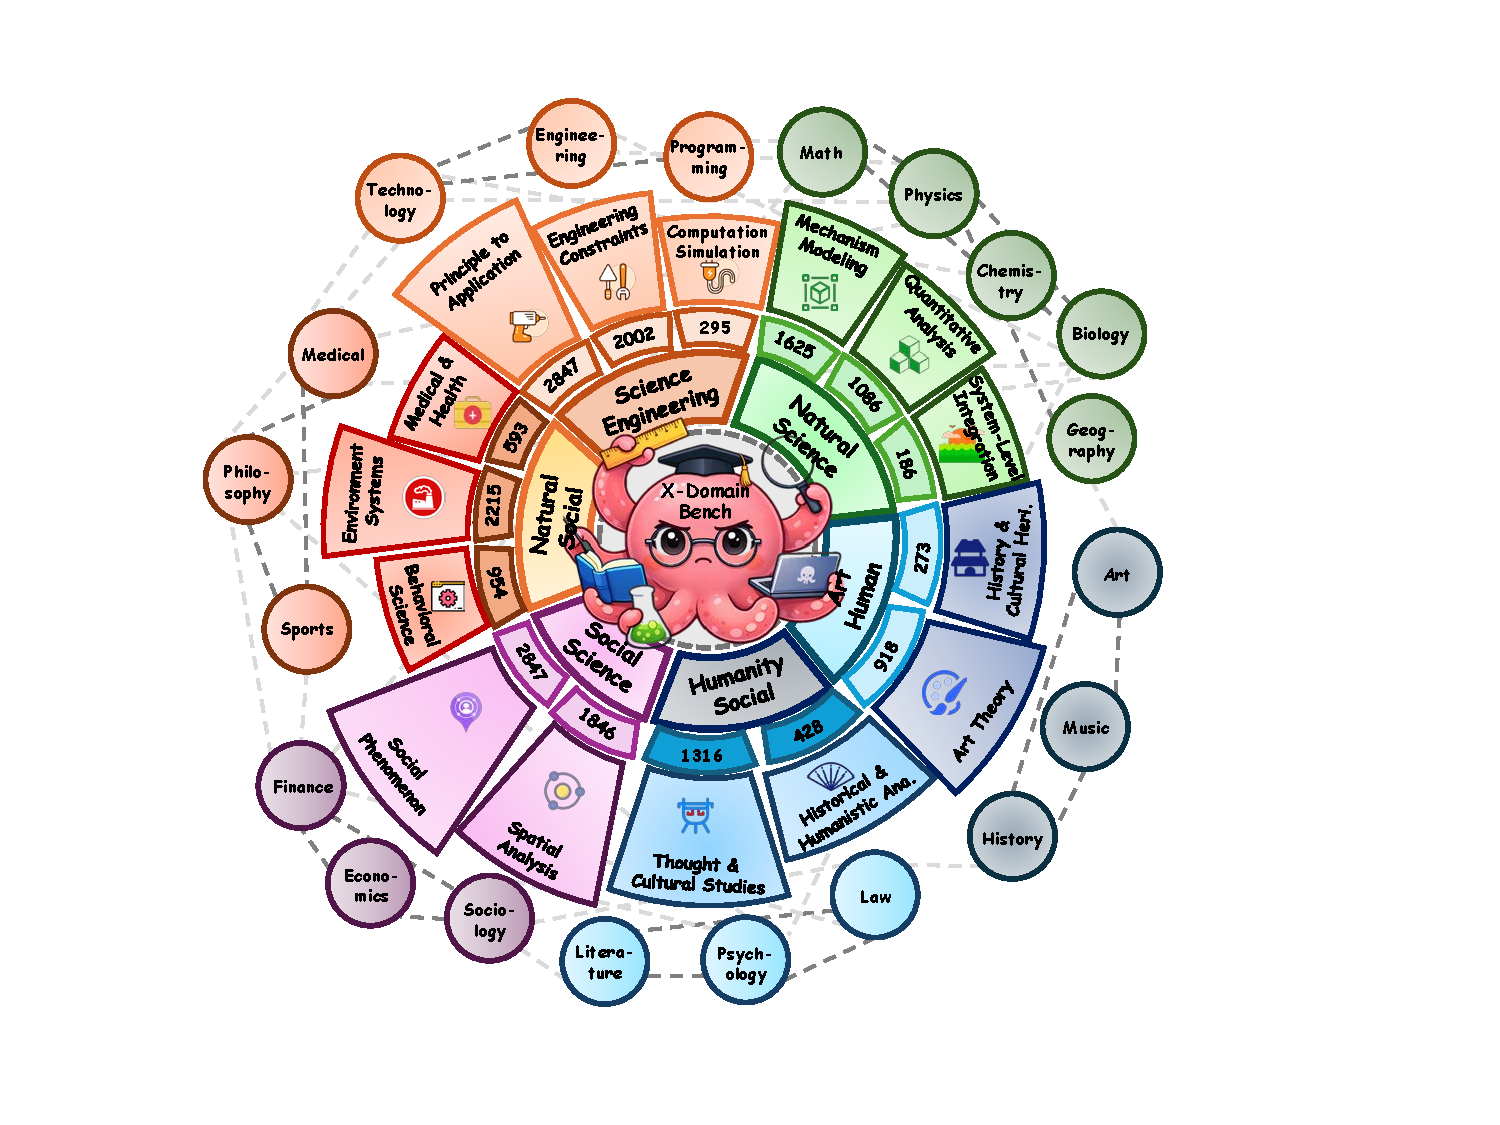
\includegraphics[width=1\linewidth]{figures/XDomainBench.pdf}
    \caption{\textbf{\textsc{XDomainBench} domain taxonomy and data scale} covering 20 domains organized into 6 major scientific categories.}
    \vspace{1mm}
    \label{fig:taxonomy}
\end{figure}

\begin{figure*}[!t]
    \centering  
    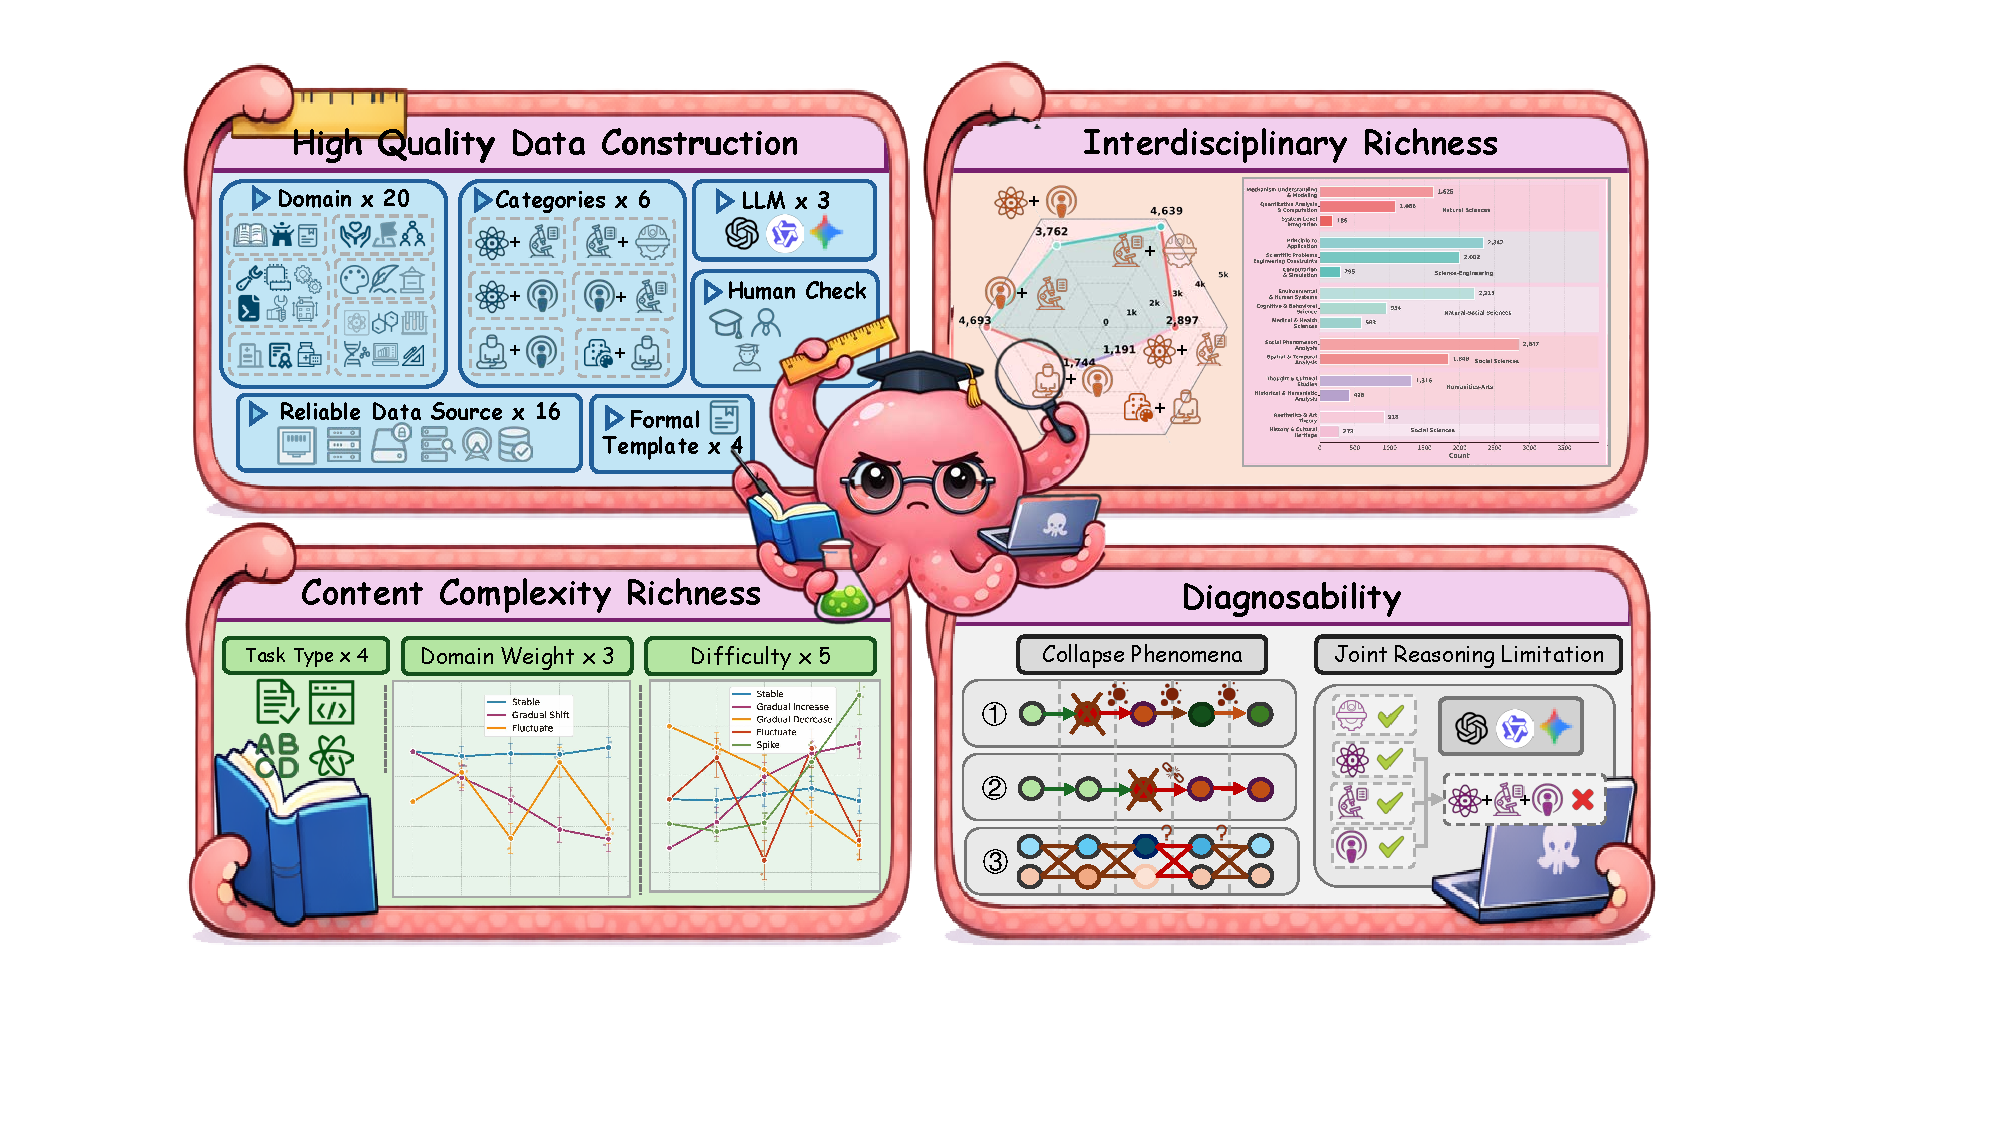
\includegraphics[width=0.98\linewidth]{figures/overview.pdf}
    % \caption{\textbf{XDomainBench at a glance. Our dataset contains multi-turn QA pairs categorized into four tasks within 20 domains. We adopt different domain compositions and various patterns of domain weights and difficulty. We support widely adopted turn- and session-level metrics to evaluate the performance of 12 LLMs.}}
    \vspace{-2mm}
    \caption{\textbf{Overview of the \textsc{XDomainBench} Framework.} The framework generates multi-turn trajectories across 20 domains and 4 task archetypes, annotated with diagnostic signals to evaluate reasoning robustness.}
    \label{fig:at_a_glance}
\end{figure*}

Despite this real-world demand, a critical evaluation gap persists. Current benchmarks struggle to capture the compositional nature of interdisciplinary scientific workflows.
Existing evaluations typically focus on static, single-domain reasoning or treat queries as isolated one-shot instances, failing to evaluate the dynamic integration and cross-domain composition required as a research trajectory evolves.
Furthermore, they lack a structured construction of interdisciplinary scenarios, making it difficult to diagnose \emph{whether failures stem from missing domain knowledge or limitations in joint reasoning}.
%Consequently, we lack a systematic diagnosis of how LLMs behave while tackling coupled constraints from multiple disciplines simultaneously and, more importantly, why their reasoning degrade.
Consequently, we lack a systematic understanding of how and why LLMs degrade when multiple scientific constraints collide.

To bridge this gap, we introduce \textsc{XDomainBench}, a diagnostic framework designed to stress-test compositional generalization in scientific reasoning as shown in Figure \ref{fig:taxonomy}.
We formalize scenario construction through two controllable dimensions: 
\textbf{(i) Composition Order}: the number of distinct domains involved, measuring the \textit{breadth} of integration.
\textbf{(ii) Mixture Structure}: the logical dependency among domains within a session, measuring the \textit{depth} of joint reasoning.
Unlike static datasets, \textsc{XDomainBench} operates within a standardized interactive controller, transforming reasoning tasks into dynamic trajectories.
% \textbf{(i) Composition Order} of distinct domains involved; and 
% \textbf{(ii) Mixture Structure} controlling how questions can exhibit varying degrees of reliance on knowledge from different domains \cite{lake2018generalization,keysers2020measuring}.
% This formalization allows us to construct a diagnostic benchmark that scales from single-discipline baselines to high-order compositions, all within a standardized interactive controller.
% 
%%这里需要一张 Table~\ref{tab:comparison}：Table~\ref{tab:comparison}: Comparison of XDomainBench with existing scientific and agentic benchmarks. Key dimensions: (1) Knowledge Composition Control (Is mixed-domain explicit?), (2) Interaction Type (Multi-turn?), (3) Diagnostic Signals (Trajectory analysis?). XDomainBench should be the only one checked for Composition Control.]%%
%Furthermore, \textsc{XDomainBench} probes reasoning robustness under composition 
By annotating each session with \textbf{trajectory-level signals} (e.g., difficulty fluctuations and domain-mixture shifts), we can move beyond simple accuracy scores to diagnose exact failure mechanisms. 
In summary, \textsc{XDomainBench} is characterized by the following key features as shown in Figure \ref{fig:at_a_glance}:
\begin{itemize}
    \item \textbf{Interdisciplinary richness}: We formalize dataset construction through composition order and mixture structure, enabling systematic control over interdisciplinary reasoning complexity and releasing \textsc{XDomainBench} with \textbf{8,598} interactive sessions across \textbf{20} domains and \textbf{4} task categories.
    \item \textbf{Content complexity richness}: We construct sessions with 8 realistic trajectory patterns covering difficulty and domain-mixture dynamics, approximating AI4S-style interactive reasoning scenarios1 with controlled complexity evolution.
    \item \textbf{Diagnosability}: We provide rich trajectory-level diagnostic annotations linking performance degradation to 3 interpretable failure mechanisms, enabling systematic diagnosis of reasoning collapse.
\end{itemize}

Our extensive experiments demonstrate a systematic reasoning collapse as composition order increases: accuracy drops from 38.7\% to 27.1\% as composition order increases, with degradation accelerating non-linearly at higher orders. This collapse stems from two root causes: \textbf{\textit{(i)}} direct complexity overhead by domain composition, and \textbf{\textit{(ii)}} indirect interaction-amplified failures, where trajectory patterns trigger error accumulation, reasoning breaks, and domain confusion, ultimately leading to session collapse.


% Artificial Intelligence for Science (AI4S) is rapidly reshaping how scientific knowledge is produced and consumed, with breakthroughs that increasingly emerge from \emph{integrating} heterogeneous evidence, tools, and domain theories across disciplinary boundaries (e.g., biology -- chemistry -- physics)~\cite{jumper2021highly,zheng-etal-2025-automation}. In parallel, Large Language Models (LLMs) are becoming a general-purpose interface for access, synthesis, and reasoning about scientific knowledge. These models range from scientific foundation models trained on scholarly corpora~\cite{taylor2022galactica} to agentic systems that combine language with tool use in complex workflows~\cite{schick2023toolformer,yao2023react}. These trends suggest a compelling opportunity: \emph{using LLMs to support interdisciplinary scientific reasoning in realistic, interactive settings}.

% Large Language Models (LLMs) are rapidly evolving into a general-purpose interface for accessing, synthesizing, and reasoning about scientific knowledge. These models range from scientific foundation models trained on scholarly corpora to agentic systems that integrate tool workflows for complex tasks. These trends indicate a compelling direction: using LLMs to facilitate interdisciplinary scientific reasoning in realistic, interactive settings.


% % 介绍现有的基准：这里要介绍与我们工作有关的benchmark

% To evaluate the progress of models within this evolving landscape, several benchmarks have been developed to measure specific facets of high-level reasoning and interaction. \citet{rein2024gpqa}~introduces a multiple-choice question benchmark at the graduate level, where domain-experts achieve approximately 65\% accuracy without access to external resources, and questions are designed to be extremely difficult to solve via web search. KnowMT-Bench benchmarks the ability of models to handle knowledge-intensive long-form question answering within multi-turn interactions, emphasizing factual depth and coherence. MINT evaluates how well LLMs solve tasks through multi-turn interactions with tools and natural language feedback, focusing on iterative reasoning and self-correction. FollowBench provides a multi-level, fine-grained framework to measure how strictly models adhere to complex, multi-layered constraints within instructions. MultiChallenge is designed to push the limits of frontier LLMs by challenging them with complex, long-range multi-turn conversations and robust interaction hurdles.

% % 引出但现有benchmarkdomain的多样性不足，且没有考虑到多轮对话中问题难度变化的动态场景

% % However, deploying LLMs for interdisciplinary science faces two fundamental obstacles. First, high-quality cross-domain data are scarce: interdisciplinary problems often require aligned, multi-source evidence and precise evaluation targets, which hinder both scalable training and reliable benchmarking~\cite{zhang-etal-2024-comprehensive-survey,rein2024gpqa}. Second, the complexity of multidisciplinary knowledge extends beyond a simple accumulation of facts; it introduces inherent logical constraints and paradigm conflicts that can lead to performance degradation during dynamic interactions~\cite{zheng-etal-2025-automation,liu-etal-2024-lost}. Constrained by these challenges, despite growing interest in scientific reasoning benchmarks~\cite{lu2022learn}, existing research remains largely confined to single-domain or weakly cross-domain, static, one-shot tasks~\cite{hendrycks2021mmlu,srivastava2022beyond,liang2022helm}. Consequently, current evaluation frameworks have yet to systematically characterize the capability boundaries and degradation mechanisms under realistic, high-dimensional knowledge compositions. 

% % 现有的评估基准在衡量模型真实性能方面仍存在显著局限。首先，受限于领域覆盖度与样本规模，现有数据集普遍存在多样性匮乏的问题，从而缺少评测模型在未知或混合场景下的表现。其次，数据集整体复杂度较低，样本难度分布过于单一，且缺乏系统性的难度梯度设计。这种缺失使得模型在训练与评估过程中，无法模拟真实环境中由浅入深的动态挑战。此外，由于跨领域知识比例难以精准调控，导致模型在知识迁移与泛化能力评估上呈现出不可预测性。因此，现有的评估体系难以精准探测大语言模型在复杂现实场景下的能力边界。

% However, existing evaluation benchmarks still have significant limitations in measuring the performance of models. First, due to constraints in domain coverage and sample scale, current datasets generally suffer from a severe lack of diversity, making it difficult to assess model performance in cross-domain scenarios. Second, the overall complexity of these datasets remains relatively low, with overly uniform difficulty distribution and a lack of systematic difficulty gradient design. This absence prevents the training and evaluation process from simulating the real-world dynamic challenges that progress from simple to complex. Furthermore, because the proportion of cross-domain knowledge is difficult to precisely control, the evaluation of models' knowledge transfer and generalization capabilities becomes unpredictable. As a result, the current evaluation system struggles to accurately detect the capability boundaries of LLM in complex real-world scenarios.

% % However, deploying LLMs for interdisciplinary science faces two fundamental obstacles. First, \textbf{high-quality cross-domain data} are scarce and difficult to curate: interdisciplinary problems often require aligned, multi-source evidence and precise evaluation targets, which limit both scalable training and reliable benchmarking~\cite{zhang-etal-2024-comprehensive-survey,rein2024gpqa}. Second, \textbf{multi-disciplinary knowledge} extends beyond a simple union of facts, introduces coupled constraints (e.g., unit/scale consistency, mechanistic compatibility) and paradigm conflicts that can induce systematic failure modes during interactive use~\cite{zheng-etal-2025-automation,liu-etal-2024-lost}. Despite growing interest in scientific reasoning benchmarks~\cite{lu2022learn,rein2024gpqa}, most existing evaluations still emphasize single-domain or weakly cross-domain, largely static one-shot settings~\cite{hendrycks2021mmlu,srivastava2022beyond,liang2022helm}, leaving the \textbf{capability boundaries} and \textbf{degradation mechanisms} under realistic cross-domain compositions under-characterized.

% % A key missing element in existing evaluations is that real scientific work is inherently \emph{interactive}, where hypotheses are iteratively refined, intermediate results feed back into subsequent questions, and evidence from different disciplines must be reconciled across multiple turns~\cite{yao2023react,liu2023agentbench}. In such settings, model behavior can degrade nonlinearly as context grows with difficulty or becomes compositionally complex, known as a phenomenon increasingly documented in long-context and stress-test evaluations~\cite{bai-etal-2024-longbench,liu-etal-2024-lost,kiela-etal-2021-dynabench}. Meanwhile, from a learning-theoretic perspective, cross-domain reasoning naturally demands \emph{compositional generalization}, which is the ability to recombine learned primitives across novel compositions. This regime has long been recognized as both critical and challenging for neural sequence models~\cite{lake2018generalization}. These observations motivate a more targeted question for AI4S: 

% % \begin{center}
% %     \emph{When disciplines intersect and compose within an interactive session, where do LLMs begin to degrade, and why?}
% % \end{center}

% \noindent To answer this, we introduce \textsc{XDomainBench}, a diagnostic benchmark for \textbf{interactive interdisciplinary scientific reasoning in high-dimensional knowledge compositions}. Our key design feature is the formalization of a \emph{knowledge-composition space}: we characterize a session as drawing from a mixture of domains and conceptualize ``high-dimensionality'' through (i) the \emph{composition order} (the number of distinct domains involved) and (ii) the \emph{mixture structure} (the distribution of domain contributions, quantified by measures such as entropy). The design enables controlled scaling from single-domain to cross-domain compositions while maintaining a realistic interactive workflow. \textsc{XDomainBench} further implements comprehensive dialogue workflows that simulate cross-disciplinary practice and evaluate models within a common interactive setting with memory and configurable general reasoning procedures. Figure~\ref{fig:at_a_glance} provides an overview of \textsc{XDomainBench}, including the controllable composition-space axes, session construction, and the diagnostic trajectories utilized for mechanism-oriented analysis.

% Empirically, we find that increasing compositional dimensionality and mixture complexity leads to substantial declines in both reasoning performance and efficiency, revealing a systematic \emph{reasoning collapse} as disciplines combine. Beyond reporting aggregate drops, we perform mechanism-oriented diagnosis and show that degradation correlates with (a) integrative reasoning difficulty induced by high-dimensional compositions and (b) interactive-session effects such as difficulty-trajectory fluctuations and domain-mixture shifts, which amplify error accumulation and progressively contaminate memory across turns~\cite{bai-etal-2024-longbench,liu-etal-2024-lost}. These results reveal a previously under-measured fragility in current LLMs within realistic AI4S workflows, highlighting that ... that are not accounted for in existing benchmarks. 


% %高维，跨域，reasoning，可控，可测量的，形容词有点多。得选出我们的特点。

% % \paragraph{Contributions.}
% In summary, this paper makes the following contributions: 
% \begin{itemize}
%     \item We formalize a \textbf{knowledge-composition space} for interdisciplinary science, making ``high-dimensional'' cross-domain reasoning controllable and measurable via composition order and mixture structure.
%     \item We build \textsc{XDomainBench}, a \textbf{diagnostic benchmark} that simulates realistic interactive cross-disciplinary scientific workflows, enabling controlled scaling from single-domain to high-order compositions.
%     \item We provide systematic evaluations and diagnoses, showing that \textbf{LLMs exhibit performance degradation as compositions grow}. We characterize \textbf{degradation mechanisms} tied to integrative difficulty and interactive-session dynamics, motivating robust and adaptive reasoning for real AI4S use.
%     % 这里可以是我们实验结果总结出的结论
% \end{itemize}